\section{Different approaches on privacy-friendliness}
In a world of constant data exchanges between different entities, it might be useful to develop methods not only to protect data during the transit as encryption classically aims to, but also when in possession of an entity that should not be able to read all of that data. This is of particular interest for computation outsourcing where a specific data-set has to be processed by an external entity that should not be able to infer anything more than what is asked from it. Furthermore, it might even be wished that one or more external entities might not be able to read the output of their computations; it should solely be readable by the original owner(s) of the data. This is of particular interest for the --- now everywhere --- cloud solutions. A protocol that respects the private character of data when treated by other entities than the owner is called \emph{privacy-friendly} or \emph{privacy-preserving}. There are different approaches to privacy-friendliness and for the sake of completeness, hereafter follows a short survey, which also justifies our choice.

\subsection{Differential privacy}
Instead of encrypting all the data, one could alternatively directly address the core problem of why we want the data encrypted: to prevent other parties to get any sensitive information contained in the data. In the case that will interest us in this thesis, we will be in possession of a lot of data from personal users which is confidential and can therefore not be traced back to the user. In 2009, Netflix launched the Netflix prize on data recommendation: the first group to improve the recommendation score of Netflix by 10\% or more would win 1.000.000\$. They provided a data-set to let the participants train their models. They also took care of anonymizing the data before they made it accessible. However, Narayanan and Shmatikov showed how they could re-identify a lot of the users by using the scores of the users on IMDb~\cite{Narayanan2006HowDataset}. \emph{Differential privacy} addresses this problem by adding noise to the data and thereby achieving a better anonymization~\cite{Dwork2008DifferentialResults}. In this way, the data is still usable for statistical models but cannot be used to identify anyone as easily as before. Still, differential privacy is limited by the fundamental and intrinsic relation between anonymization and statistical relevance. One cannot obtain the first without inevitably having an influence on the second one, and reciprocally.

\subsection{Homomorphic encryption}
Differential analysis is a statistical approach of anonymity, but there also exist some cryptographic approaches, where the external entity is not able to read the results of what it produces. It is possible to construct a protocol with one or more third parties in a way that they cannot possibly learn anything from what they are receiving nor what they are sending back: the information is processed in an encrypted and not a clear form. Encryption schemes that allow mathematical operations to be executed on the encrypted data are called \emph{homomorphic} and were first proposed by Rivest et al. in 1978~\cite{Rivest1978}. For example, the RSA encryption scheme preserves the multiplication over the encrypted data~\cite{Rivest:1978:MOD:359340.359342}. The RSA encryption scheme is given by $\mathscr{E}(m)=m^e \mod N$. We thus have $\mathscr{E}(m_1) \cdot  \mathscr{E}(m_2) = \left(m_1^e \mod N \right)\left(m_2^e \mod N \right) = \left(m_1m_2\right)^e \mod N = \mathscr{E}(m_1m_2)$. Unfortunately, this property is only true for multiplication and is therefore quite limited in its applications. We therefore refer to RSA as a \emph{somewhat-homomorphic} encryption scheme (SHE). When all mathematical operations are possible, we say from the encryption scheme that it is \emph{fully-homomorphic} (FHE). Up to now, only some schemes based on finite fields possess this property. 

The most accomplished method up to now is called the \emph{Approximate Eigenvector Method} and is based on the \emph{Learning With Errors} (LWE) encryption scheme. This scheme is also known for still being secure in a post-quantum era. If $C_1$ and $C_2$ are two matrices with common eigenvector $s$, we notice that the sum or multiplication of their respective eigenvalues $m_1$ and $m_2$ corresponds to the eigenvalue of the sum or multiplication of $C_1$ and $C_2$ with respect to $s$. The eigenvector act as a private key and the eigenvalues as the secret messages. The scheme is thus fully homomorphic. However, eigenvectors are easy to find and the scheme is thus also insecure. To resolve this, the method uses approximate eigenvectors $sC=ms+e\approx ms$ which is known to be still solvable in finite fields under a few assumptions about the error $e$~\cite{Regev:2005:LLE:1060590.1060603}.

\subsection{Multi-party computation}
When different parties participate to the input, the homomorphic encryption described above cannot be used anymore: all parties have to share the same secret key which keeps their data private with respect to the third party, but not to each other. Multi-party computation addresses this problem. Furthermore, it also allows the parties to compute a common function on their private inputs without needing one or more third parties. 

More concretely, let us now imagine a problem where the goal is to compute some common function $f$ over private inputs $x_i$. In other words, we want to compute $f\left(x_1, \, \ldots, \, x_n\right) = \left( y_1, \, \ldots , \, y_n\right)$ where each input $x_i$ is privately provided by party $P_i$, which ultimately learns $y_i$ and nothing more: not the other outputs, nor the other inputs. A first naive implementation would be to trust a third party to privately receive each player's input, computing the function and privately communicating the corresponding responses to the concerned parties. However, it also possible to obtain the same results without the trust of a third party, where only the parties are participating to the protocol. This is called \emph{multi-party computation} (MPC) also referred to as \emph{secure multi-party computation} (SMC). This approach has been chosen to solve our problem and will be described more extensively here under and in the next section.

Multi-party computation originated with the toy example presented by Yao in 1982~\cite{Yao1982ProtocolsComputations} that is now known as the \emph{Millionaire's Problem}: two millionaires both want to know who is richer, but none of them wants to disclose their fortune to the other one nor trust a third party. Other applications of MPC may concern electronic voting or solutions of private-data as a service (PDaaS). The different methods defined here under have a common general way of working. The computation is done in rounds: each party computes some algorithms on its own and then exchange som information with the other parties. The exchanges do not happen continuously, but all together in what is called a round. A new computation phase can then take place followed by a next exchange phase.


\subsubsection{Bit-wise decomposition}
There basically exist two big families of multi-party computation protocols and each of them is based on a different cryptographic primitive. A cryptographic primitive is the basic block or idea on which the whole protocol is based. The first one described here decomposes every operation into a boolean circuit and every value into its bits, hence its name. The cryptography takes place at bit-level. The two multi-party protocols described here under use the idea of oblivious transfer, which is first described.

\paragraph{Oblivious transfer}
The idea behind \emph{oblivious transfer} originally described by Rabin in 1981 \cite{Rabin1981HowTransfer.} is the transfer of an certain information in possession of a first party and asked by a second party, without the first party knowing which information has been transferred. Hence the name oblivious, or alternatively, unconscious. Different protocols exist and are all based on the \emph{RSA scheme}. 

The most common version is the \emph{1-2 oblivious transfer} and goes as follows~\cite{Even1985AContracts}: Alice is in possession of two messages $m_0$ and $m_1$ and Bob wants to get message $m_p$. Alice first generates a set of private key $d$ and public key $(N,e)$ and sends two random messages $x_0$ and $x_1$ to Bob. He then generates a random message $k$ and encrypts it with the $x$ corresponding to the wanted message: $v = \left(x_p + k^e\right) \mod N$ and sends it to Alice. She then recovers both $k$ without knowing which one corresponds to Bob's original one: $k_i = \left(v-x_i^d\right) \mod N$. These $k_i$ then serve to encrypt the messages which are finally sent to Bob $s_i = m_i+k_i$. Bob can then only decrypt the wanted message $m_p = s_p-k$. 

This protocol has been generalized to more than two parties \cite{Ishai1997PrivateApplications,Shankar2008AlternativeTransfer,Tassa2011GeneralizedSharing}.

\paragraph{Yao's garbled circuits}
\begin{wrapfigure}[16]{R}{0.5\textwidth}
\begin{center}
    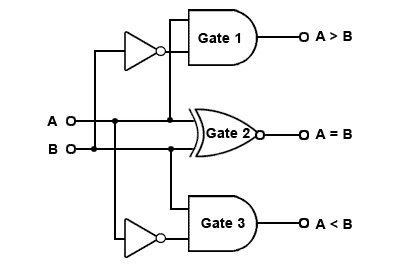
\includegraphics[width=.45\textwidth]{parts/chap-3/img-3/yao-comp.jpg}
    \caption[The digital comparator]{The digital comparator is the boolean circuit used to solve Yao's millionaire problem.} 
    \label{privacy:yao-comp}
\end{center}
\end{wrapfigure}
\emph{Garbled circuits} (GC) were first introduced by Yao in 1986 and are now one of the most efficient solutions for generic secure two-party computation~\cite{Yao1986HowSecrets}. A function has to be decomposed into a boolean circuit consisting of two-input gates (e.g. XOR and AND). Let's consider the simplest example of evaluating an AND-gate between Alice and Bob. Alice first generates a different random sequence --- also called \emph{labels} --- for each possible value of each input --- also called \emph{wires} --- and output. In the truth table, the output are then symmetrically encrypted with the hash of each corresponding input. These four resulting cyphertexts are then randomly permuted --- hence the name \emph{garbled} --- and sent to Bob. The garbling of an AND-gate is illustrated at table~\ref{tab:ang-garb}. Once Bob receives the garbled gate, he then asks Alice for her label. As they have been randomly chosen, she can send it to him without him possibly knowing what value it corresponds to. Afterwards, he also needs to know the label of his input. This part is a bit more tricky and is solved using the previously described \emph{oblivious transfer}. Bob can now compute the hash of the two labels and decrypt each element of the garbled gate until he finds one corresponding with the garbled gate he received from Alice. He can then reveal the value to Alice or she can reveal the mapping of the garbling. The same principle can be used on a multi-gate circuit by garbling the sole end result.

\begin{figure}
        \begin{subfigure}[b]{.32\textwidth} 
            \centering 
            \begin{tabular}{IC{.6cm}|C{.6cm}IC{1.3cm}I}
            \hlineI
            A & B & output \\ \hlineI
            0 & 0 & 0  \\ \hline
            1 & 0 & 0 \\ \hline
            0 & 1 & 0 \\ \hline
            1 & 1 & 1 \\ \hlineI
            \end{tabular}
            \caption{Truth table.} 
        \end{subfigure}
        \hfill
        \begin{subfigure}[b]{.32\textwidth} 
            \centering 
            \begin{tabular}{IC{.6cm}|C{.6cm}IC{1.3cm}I}
            \hlineI
            A & B & output \\ \hlineI
            $x_A^0$ & $x_B^0$ & $x_{\textnormal{output}}^0$ \\ \hline
            $x_A^1$ & $x_B^0$ & $x_{\textnormal{output}}^0$ \\ \hline
            $x_A^0$ & $x_B^1$ & $x_{\textnormal{output}}^0$ \\ \hline
            $x_A^1$ & $x_B^1$ & $x_{\textnormal{output}}^1$ \\ \hlineI
            \end{tabular}
            \caption{Labelled truth table.} 
        \end{subfigure}
        \hfill
        \begin{subfigure}[b]{.32\textwidth}
            \centering 
            \begin{tabular}{IC{3.2cm}I}
            \hlineI
            output \\ \hlineI
            $\mathscr{E}_{H\left(x_A^1|x_B^0\right)}\left(x_{\textnormal{output}}^0\right)$ \\ \hline
            $\mathscr{E}_{H\left(x_A^1|x_B^1\right)}\left(x_{\textnormal{output}}^1\right)$ \\ \hline
            $\mathscr{E}_{H\left(x_A^0|x_B^0\right)}\left(x_{\textnormal{output}}^0\right)$ \\ \hline
            $\mathscr{E}_{H\left(x_A^0|x_B^1\right)}\left(x_{\textnormal{output}}^0\right)$ \\ \hlineI
            \end{tabular}
            \caption{Garbled output.} 
        \end{subfigure}
        \captionof{table}{Garbling of the AND-gate.}
        \label{tab:ang-garb}
\end{figure}

It is interesting to note that the secure evaluation of a sole AND-gate does not respect the principles of multi-party computation, by definition of the AND-gate. Indeed, if the final solution is 1, both players know their respective input value, which is thus disclosed\footnote{This is not the case for the XOR-gate as the 1-output has two corresponding inputs possible, as has the 0-output}. Therefore, the total functions evaluated cannot be injective for any input. The circuit corresponding to the Millionaire's problem is given at figure~\ref{privacy:yao-comp} and while it consists of AND-gates, the function isn't injective at all with respect to each millionaire's fortune.

This protocol executes in polynomial time, but there exist a lots of optimizations that allow to garble and evaluate the gates more rapidly~\cite{YakoubovAContents}.

\paragraph{GMW protocol}
The \emph{Goldreich-Micali-Widgerson} (GMW) protocol can be seen as an extension of garbled circuits to multiple parties using Yao's idea of using oblivious transfer~\cite{Goldreich1987HowGame}. The main principles here are based upon bit-sharing: each party shares its input bits among the $n$ players $b = \sum_{i=1\ldots n}b_i \mod 2$. Each player then processes their shares among the circuit. XOR-gates are easy as they can just addition the shares $c_i = a_i + b_i$. However AND-gates are more tricky: we can see from the decomposition that $c = a \cdot b = \sum_{i\neq j}a_ib_j+\sum_{1\leq i< j\neq n}\left(a_ib_j + a_jb_i \right) \mod 2$. Each party will then have to compute $a_ib_i+ \sum_{i\neq j}\left( a_ib_j + a_jb_i\right)$. As for the XOR-gate, the first part is trivial to evaluate, however, the second cannot be computed by party $i$ without more information from party $j$. This is solved by using a variant of garbled circuits with oblivious transfer between parties $i$ and $j$.

\subsubsection{Avoiding bit-wise decomposition}
Alternatively to boolean circuits, arithmetic circuits can also be used for multi-party computation. The problem of bit-wise decomposition and the use of the boolean circuit transcription of the function that we jointly want to evaluate, is their expensiveness. Indeed, a simple operation can rapidly lead to a lot of gates. For example, let's consider the addition of two numbers: for two numbers of $n$ bits, the total number of gates is $5n$ in a full adder composition. This is even worse for multiplication. Of course, some optimizations can be made, but the general number of gates is very high compared to the arithmetic circuit of the same function, where it would just be one single gate for addition and multiplication. In general, MPC over arithmetic circuits require a much higher number of rounds. Though, they seem in total more efficient for solving complex problems. Even 2-party comparisons do not seem much more efficient with garbled circuits --- for which they were originally tailored -- compared to the method described here-under~\cite{Blom2014AThesis}.

The cryptographic primitive of multi-party computation over arithmetic circuits is based upon \emph{secret sharing}. Each party computes its own version of the circuit with the shares of the different parties. At the end of the circuit processing, each party has a share of the final output, which can then be put together to obtain the final output. We first have to define a way for a party to share its secret among $n$ parties.

\paragraph{Additive secret sharing}
The simplest idea is just to divide the secret $a$ in $n$ shares $a_i$ using a simple summation: $a = \sum_{i=1 \ldots n}a_i$. This cryptographic primitive is often referred to as the \emph{linear secret sharing scheme} (LSSS). However, doing it in this manner allows the shares to release some information about the secret, as the shares are not random and strongly depend on the secret. They are two solutions to this problem and the first one is to consider additive sharing over $\mathbb{Z}_q$. The sharing now becomes $a = \sum_{i=1\ldots n}a_i \mod q$ which solves the problem, as the shares can now really be chosen at random. The other solution is over $\mathbb{Z}$ and consists of choosing a sufficiently large interval in which the shares are chosen to dilute sufficiently the statistical information about the secret, typically $a_i \in \left[-A2^\kappa,A2^\kappa\right]$ with $A$ the size of the interval of the secret $a \in \left[-A,A\right]$. The size of $a$ is of maximum bit-length $k$ and we therefore also refer to $\mathbb{Z}_k$ alternatively the interval.

Another consequence of this scheme is that all parties are vital to the recovery of secret, as the loss of one secret prevents us to reconstruct the secret or any statistical information about it. The scheme does not tolerate the loss or treason of one party and is therefore very sensitive to any failure or malicious player. This problem is solved by polynomial secret sharing.

\paragraph{Polynomial secret sharing}
The idea of polynomial sharing was originally proposed by Shamir in 1979 \cite{Shamir1979HowSecret}. This cryptographic primitive is often referred to as \emph{Shamir secret sharing}. It allows $n$ parties to share a secret in such a way that any subset of $t+1$ parties can later reconstruct the secret, but any subgroup of maximum $t$ parties cannot do so. The scheme is based on the single fact that for any polynomial of degree $d$, any subset of $d+1$ or more different points can be used to reconstruct the polynomial completely whereas any subset of at most $d$ points lefts us with an infinite number of possibilities.

The scheme goes as follows. The party that wants to share its secret first constructs a polynomial of degree $t$:
\begin{equation}
    h(z) = a + \sum_{i=1}^t b_i z^i,
\end{equation}
with secret $a$ random coefficients $b_i$. For the same reasons as for additive secret sharing, the coefficients can either be chosen in $b_i \in \mathbb{Z}_q$ (which also leads to the consideration of polynomial $h(z) \mod q$ instead), either in the interval $b_i \in \left[-A2^\kappa,A2^\kappa\right]$.

We verify that $h(0)=a$ and distribute shares $a_i$ to each party $i$ as follows $a_i=h(i)$. $t+1$ parties can now reconstruct the polynomial together using e.g. Lagrange's polynomials and compute $f(0)$ to recover the secret share. An interesting property is that the recovery can be done as a simple linear combination. Indeed, we have
\begin{eqnarray}
    h(0) &=& \sum_{i=1}^{n} l_i(0)h(i) \\
    a &=& \sum_{i=1}^{n} r_ia_i,
    \label{eqn:recover-secret}
\end{eqnarray}
where $r = \left(r_1, \ldots , r_n\right) = \left(l_1(0), \ldots , l_n(0)\right)$ is called the \emph{recombination vector} with $l_i(z)$ the $i$-th order Lagrange polynomial, for example
\begin{equation*}
    l_i(z) = \prod_{1\leq j \leq n,j\neq i}\frac{z-j}{i-j}.
\end{equation*}

The sum of a the elements of a recombination vector always equals 1 ($\sum_{i=1}^n r_i=1$). It can be constructed with any generating set of the polynomial space $\mathbb{Z}\left[z\right]$ (or alternatively $\mathbb{Z}_q\left[z\right]$), as long all parties use the same set.